\documentclass{article}%
\usepackage[T1]{fontenc}%
\usepackage[utf8]{inputenc}%
\usepackage{lmodern}%
\usepackage{textcomp}%
\usepackage{lastpage}%
\usepackage[head=40pt,margin=0.5in,bottom=0.6in]{geometry}%
\usepackage{graphicx}%
%
\title{\textbf{Comisionado de la Acnur llegó a Colombia para ayudar a los venezolanos}}%
\author{EFE}%
\date{07/10/2018}%
%
\begin{document}%
\normalsize%
\maketitle%
\textbf{URL: }%
http://www.el{-}nacional.com/noticias/mundo/comisionado{-}acnur{-}llego{-}colombia{-}para{-}ayudar{-}los{-}venezolanos\_254722\newline%
%
\textbf{Periodico: }%
EN, %
ID: %
254722, %
Seccion: %
Mundo\newline%
%
\textbf{Palabras Claves: }%
Colombia, Diáspora, ONU\newline%
%
\textbf{Derecho: }%
18%
, Otros Derechos: %
CONTEXTO%
, Sub Derechos: %
NO\_TIENE%
\newline%
%
\textbf{EP: }%
NO\newline%
\newline%
%
\textbf{\textit{El encargado del ente que ofrece apoyo a los refugiados indicó que se debe planificar cómo ayudar mejor al gobierno colombiano, que continúa recibiendo migrantes desde Venezuela~}}%
\newline%
\newline%
%
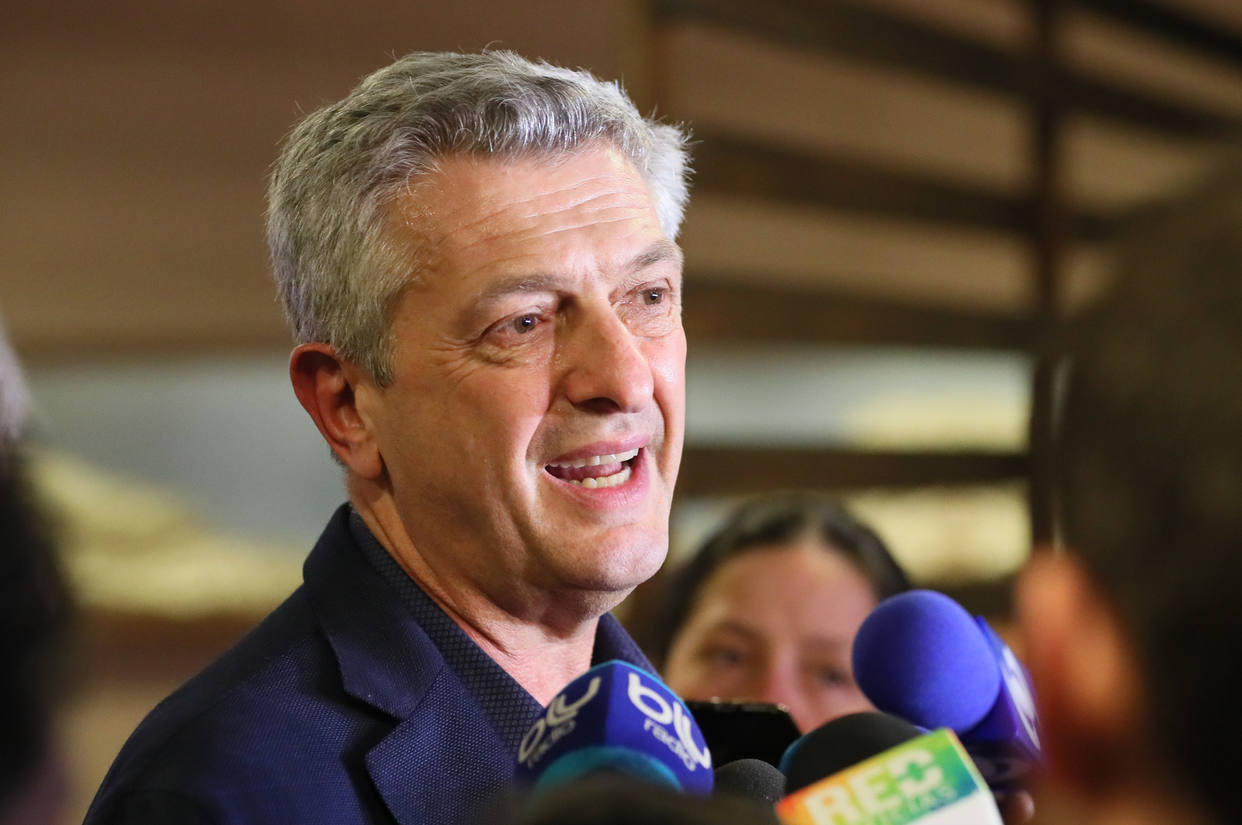
\includegraphics[width=300px]{185.jpg}%
\newline%
%
Filippo Grandi, alto comisionado de la Organización de las Naciones Unidas para los Refugiados, aseguró luego de llegar a Bogotá que el objetivo de su visita al país latinoamericano~es conocer de primera mano las dificultades que enfrentan los venezolanos en Colombia.%
\newline%
%
"Yo creo que es muy importante para mí~comprender los problemas concretos de los venezolanos, para planificar mejor la futura~acción de apoyo al gobierno colombiano", dijo Grandi en rueda de prensa junto al canciller de Colombia, Carlos Holmes Trujillo.%
\newline%
%
El funcionario indicó que "la preocupación principal de la ONU es que los venezolanos puedan tener instrumentos de acceso a una protección en formas diferentes y disponibles en varios países y que no estén expuestos a riesgos y peligros, especialmente las mujeres, los niños y las personas mayores".%
\newline%
%
Tanto Grandi como Trujillo resaltaron la importancia de que Acnur, junto a la Organización Internacional de las Migraciones, estableciera~una plataforma de coordinación regional y designado como representante especial a Eduardo Stein,~ex vicepresidente de Guatemala.%
\newline%
%
El comisionado resaltó que Stein deberá trabajar con los gobiernos de las naciones receptoras de venezolanos para que "el trabajo sea más eficaz, buscar recursos y desarrollar una estrategia regional, porque muchos problemas son los mismos en diferentes países".%
\newline%
%
Asimismo, el canciller colombiano agradeció la presencia de Grandi e indicó que el gobierno pretende fortalecer los mecanismos internos para enfrentar la crisis migratoria.%
\newline%
%
Holmes comentó que en los próximos días viajará a Lima y Quito para "poner en marcha la primera parte del proceso de armonización de las medidas, para hacerle frente a la situación~generada por el éxodo de venezolanos".%
\newline%
%
\end{document}